\documentclass[a4paper,12pt]{article}

\usepackage[utf8]{inputenc}
\usepackage[spanish]{babel}
\usepackage{amsmath, amssymb}
\usepackage{graphicx}
\usepackage{float}
\usepackage{booktabs}
\usepackage{xcolor}
\usepackage{listings}
\usepackage{caption}
\usepackage{fancyhdr}
\usepackage{hyperref}
\usepackage{tikz}
\usepackage{tabularx}

\hypersetup{
    colorlinks=true,
    linkcolor=blue,
    urlcolor=blue,
    pdftitle={Práctica 6 - Uso de paquetes},
}

% === Definición de colores similares a Vivado ===
\definecolor{vivadoKeyword}{rgb}{0.6,0.0,0.6}
\definecolor{vivadoComment}{rgb}{0.0,0.5,0.0}
\definecolor{vivadoString}{rgb}{0.5,0.2,0.0}
\definecolor{vivadoBackground}{rgb}{0.97,0.97,0.97}

\lstdefinelanguage{VHDL}{
    morekeywords={library, use, entity, is, port, in, out, end, architecture, of, begin, signal, if, then, else, when, others, xor, and, or, not},
    sensitive=true,
    morecomment=[l]--,
    morestring=[b]",
}

\lstset{
    language=VHDL,
    backgroundcolor=\color{vivadoBackground},
    keywordstyle=\color{vivadoKeyword}\bfseries,
    commentstyle=\color{vivadoComment}\itshape,
    stringstyle=\color{vivadoString},
    basicstyle=\ttfamily\small,
    numbers=left,
    numberstyle=\tiny,
    numbersep=5pt,
    frame=single,
    breaklines=true,
    tabsize=2,
    captionpos=b
}

\title{Práctica N°6: Uso de Paquetes}
\date{}

\begin{document}
\maketitle
\tableofcontents
\newpage

\section{Objetivos}
\label{sec:objetivos}

\subsection{Objetivo general}
Diseñar, implementar y verificar una \textbf{ALU de 4 bits} en \textbf{VHDL-2008} que utilice \textbf{paquetes} para (i) los tipos y operaciones aritméticas (\textit{add, subtract, multiply, divide}) y (ii) la \textbf{presentación en displays de 7 segmentos}, integrando todo en un único módulo \textit{top} capaz de mostrar \textbf{A} (en dos dígitos), \textbf{B} (en dos dígitos) y el \textbf{resultado} (en cuatro dígitos), con manejo explícito de \textit{flags} y del caso \textit{división por cero}, sintetizable para \textbf{Nexys A7-100T} en \textbf{Vivado 2023.2}.

\subsection{Objetivos específicos}
\begin{itemize}
  \item Definir en un paquete de tipos una \textit{API} clara: subtipos sin signo de 4 y 8 bits, el tipo enumerado de operación y un \textit{record} de banderas (\textit{carry, borrow, zero, overflow, divide\_by\_zero}) junto al \textit{record} de resultado de la ALU.
  \item Implementar en un paquete de operaciones funciones puras y combinacionales para \textbf{suma}, \textbf{resta}, \textbf{multiplicación} (8 bits) y \textbf{división} (cociente y residuo), con manejo explícito de \textbf{división por cero}; emplear exclusivamente \texttt{ieee.numeric\_std}.
  \item Diseñar un paquete de visualización para 7 segmentos: LUT \texttt{HEX$\rightarrow$7SEG} (activos en bajo) y \textbf{conversores decimales} (4 bits $\rightarrow$ 2 dígitos, 8 bits $\rightarrow$ 4 dígitos) para presentar A, B y el resultado en formato decimal.
  \item Desarrollar un \textbf{driver de multiplexado de 8 dígitos} (AN7..AN0) con frecuencia de refresco por dígito $\geq$ 1~kHz para evitar parpadeo, y puntos decimales como indicadores de error en \textit{divide by zero}.
  \item Integrar en un \textit{top} único: mapeo A$\rightarrow$AN7..AN6, B$\rightarrow$AN5..AN4, resultado
  $\rightarrow$AN3..AN0; exportar \textit{flags} a LEDs; preparar \textbf{XDC} con IOSTANDARD correcto.
  
\end{itemize}

\section{Configurar VHDL-2008 en Vivado}
\label{sec:vhdl2008}

Para evitar errores de síntesis como \texttt{OTHERS in array aggregate without constraining context} y asegurar compatibilidad con paquetes y \texttt{numeric\_std}, es indispensable fijar el estándar \textbf{VHDL-2008} tanto a nivel de proyecto como (si hace falta) por archivo.


\subsection{Forzar VHDL-2008 por archivo (si algún fichero no hereda)}
\begin{enumerate}
  \item En el \textbf{Sources}, clic derecho sobre el archivo \texttt{.vhd} problemático $\rightarrow$ \textbf{Source File Properties}.
  \item En \textbf{VHDL Language Version}, seleccione \textbf{VHDL 2008}.
  \item Aplique cambios y vuelva a sintetizar.
\end{enumerate}

\begin{figure}[H]
  \centering
  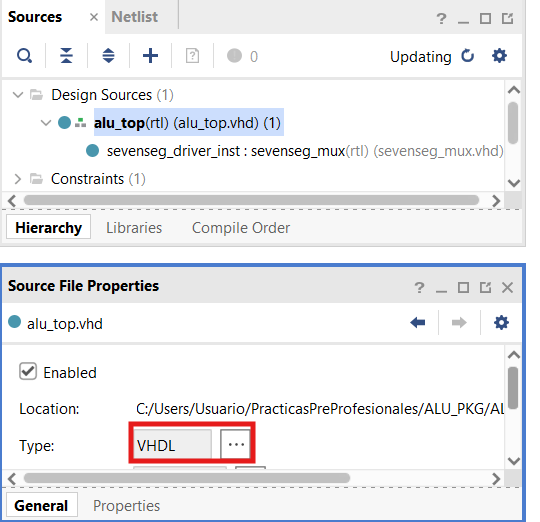
\includegraphics[width=\textwidth]{2008_1.png}
  \caption{Propiedades por archivo: forzar \emph{VHDL 2008} en un \texttt{.vhd} concreto.}
  \label{fig:vhdl2008-file}
\end{figure}

\begin{figure}[H]
  \centering
  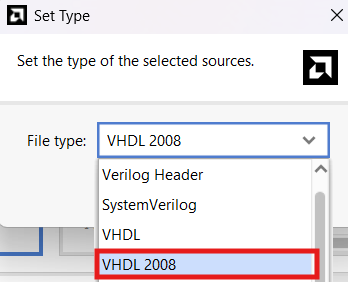
\includegraphics[width=0.8\textwidth]{2008_2.png}
  \caption{Propiedades por archivo: forzar \emph{VHDL 2008} en un \texttt{.vhd} concreto paso 2.}
  \label{fig:vhdl2008-file}
\end{figure}

\section{Marco teórico}
\subsection{Paquetes en VHDL y su utilidad}
En VHDL, un \textbf{paquete} (\textit{package}) es una unidad de diseño que agrupa \emph{declaraciones reutilizables}: tipos (\texttt{type}, \texttt{subtype}), constantes, funciones y procedimientos. Un paquete se compone de una \textbf{declaración} (\texttt{package})—donde se exponen las interfaces—y, opcionalmente, un \textbf{cuerpo} (\texttt{package body})—donde se implementan las subrutinas. Otros módulos obtienen visibilidad usando \texttt{library}/\texttt{use} (p.\,ej., \texttt{use work.mi\_pkg.all;}).

\noindent\textbf{¿Para qué sirven?} 
\begin{itemize}
  \item \textbf{Modularidad y reutilización}: centralizan tipos, constantes (p.\,ej., LUTs) y funciones comunes (p.\,ej., operaciones de ALU, conversores a 7 segmentos).
  \item \textbf{Interfaces estables}: evitan duplicación y desalineación de definiciones entre el \textit{top}, testbenches y bloques internos.
  \item \textbf{Mantenibilidad y portabilidad}: cambiar una definición en el paquete actualiza a todos los consumidores.
  \item \textbf{Buenas prácticas de síntesis}: funciones \emph{puras}, constantes bien tipadas y \textbf{sin señales ni procesos} en el paquete (solo declaraciones), favoreciendo resultados predecibles en hardware.
  \item \textbf{Parametrización} (VHDL-2008): permiten \textit{package generics} para ajustar valores globales sin tocar múltiples archivos.
\end{itemize}


\section{Descripción del código}
\label{sec:descripcion-codigo}

\subsection{Paquete \texttt{alu\_types\_pkg}}
\label{subsec:alu-types-pkg}

\begin{lstlisting}[language=VHDL,caption={Paquete de tipos y constantes para la ALU didáctica.},label={lst:alu-types-pkg}]
library ieee;
use ieee.std_logic_1164.all;
use ieee.numeric_std.all;

-- =======================
-- Paquete de tipos y constantes para la ALU didactica de 4 bits
-- Define subtipos con nombres explicitos, el conjunto de operaciones,
-- un registro de banderas (flags) y el tipo de resultado de la ALU.
-- ========================
package alu_types_pkg is
  -- Tipos base con nombres claros
  subtype unsigned_4bit_t is unsigned(3 downto 0);
  subtype unsigned_8bit_t is unsigned(7 downto 0);

  -- Conjunto explicito de operaciones
  type operation_t is (OPERATION_ADD, OPERATION_SUBTRACT, OPERATION_MULTIPLY, OPERATION_DIVIDE);

  -- Banderas de estado con nombres completos
  type flags_record_t is record
    carry_flag            : std_logic;  -- valido para suma sin signo
    borrow_flag           : std_logic;  -- valido para resta sin signo (1 = hubo prestamo)
    zero_flag             : std_logic;  -- 1 cuando el resultado relevante es cero
    overflow_flag         : std_logic;  -- p/ unsigned: ADD=carry; SUB=borrow; MUL=parte alta != 0
    divide_by_zero_flag   : std_logic;  -- 1 si B = 0 en division
  end record;

  -- Resultado de la ALU empaquetado y autoexplicativo
  type alu_result_record_t is record
    result_8bit_unsigned  : unsigned_8bit_t;   -- resultado principal de 8 bits (ADD/SUB/MUL).
    quotient_4bit_unsigned  : unsigned_4bit_t; -- cociente (DIV)
    remainder_4bit_unsigned : unsigned_4bit_t; -- residuo  (DIV)
    flags                   : flags_record_t;  -- banderas
  end record;
end package;

package body alu_types_pkg is
end package body;
\end{lstlisting}

\paragraph{Qué resuelve este paquete y por qué existe.}
Este paquete \textbf{aclara contratos} entre módulos: define \emph{qué} tamaños de datos se usarán, \emph{qué} operaciones reconoce la ALU y \emph{cómo} se reportan los resultados y estados (banderas). Al centralizar estos tipos:
(i) evitamos inconsistencias de ancho, (ii) documentamos la interfaz, y (iii) facilitamos pruebas y mantenimiento.

\paragraph{Importaciones (\texttt{library}/\texttt{use}).}
Se usan \texttt{std\_logic\_1164} para tipos lógicos y \texttt{numeric\_std} para aritmética \textbf{sin signo} y \textbf{con signo}. Elegimos \texttt{numeric\_std} (en lugar de paquetes no estándar como \texttt{std\_logic\_unsigned}) para mantener portabilidad y un comportamiento bien definido en síntesis.

\paragraph{Subtipos con semántica explícita.}
\begin{itemize}
  \item \texttt{unsigned\_4bit\_t} $\rightarrow$ operandos de la ALU (\(A,B\)), rango \(0..15\).
  \item \texttt{unsigned\_8bit\_t} $\rightarrow$ resultados que pueden exceder 4 bits (p.\,ej., \(15\times15=225\)), rango \(0..255\).
\end{itemize}
Usar \textit{subtypes} en lugar de \texttt{unsigned(3 downto 0)} “a pelo” obliga a una \textbf{consistencia de tamaños} y mejora la legibilidad.

\paragraph{Tipo enumerado de operación \texttt{operation\_t}.}
Define el \textbf{dominio de operaciones} de la práctica:
\texttt{ADD}, \texttt{SUBTRACT}, \texttt{MULTIPLY}, \texttt{DIVIDE}.  
Ventaja: el \texttt{top} y los testbenches pueden \emph{seleccionar} la operación con nombres semánticos en lugar de literales numéricos, reduciendo errores.

\paragraph{Banderas de estado \texttt{flags\_record\_t}.}
Las banderas capturan \textbf{condiciones relevantes} por operación. Úsalas como telemetría y para evaluación:
\begin{center}
\begin{tabular}{@{}lllll@{}}
\toprule
\textbf{Bandera} & \textbf{Tipo} & \textbf{Se activa cuando} & \textbf{Aplica en}  \\
\midrule
\texttt{carry\_flag} & \texttt{std\_logic} & Suma excede 4 bits & ADD  \\
\texttt{borrow\_flag} & \texttt{std\_logic} & \(A<B\) en resta & SUBTRACT  \\
\texttt{zero\_flag} & \texttt{std\_logic} & Resultado relevante es 0 & Todas  \\
\texttt{overflow\_flag} & \texttt{std\_logic} & Convención unsigned & ADD/SUB/MUL \\
\texttt{divide\_by\_zero\_flag} & \texttt{std\_logic} & Divisor \(B=0\) & DIVIDE \\
\bottomrule
\end{tabular}
\end{center}

\paragraph{Registro de resultado \texttt{alu\_result\_record\_t}.}
Estructura canónica que \textbf{agrega todo lo que un consumidor necesita}:
\begin{enumerate}
  \item \texttt{result\_8bit\_unsigned}: canal principal para ADD, SUB y MUL; permite visualizar tanto la parte baja como la alta (si existe).
  \item \texttt{quotient\_4bit\_unsigned} y \texttt{remainder\_4bit\_unsigned}: salidas claras para DIV (evita ambigüedades).
  \item \texttt{flags}: el \emph{estado} de la operación viaja junto al dato, simplificando verificación y depuración.
\end{enumerate}
Para DIV, además se especifica que \texttt{result\_8bit\_unsigned} se empaqueta como \([remainder][quotient]\) (nibble alto y bajo). Esto facilita inspección rápida en simulación/ILA sin tener que mirar múltiples señales.

\newpage

\subsection{Paquete \texttt{alu\_ops\_pkg}}
\label{subsec:alu-ops-pkg}

\begin{lstlisting}[language=VHDL,caption={Operaciones combinacionales de la ALU (unsigned).},label={lst:alu-ops-pkg}]
library ieee;
use ieee.std_logic_1164.all;
use ieee.numeric_std.all;

use work.alu_types_pkg.all;

-- ===============================
-- Paquete de operaciones puras de la ALU (combinacionales, didacticas).
-- Todas trabajan en UNSIGNED (sin signo) para mantener la practica simple.
-- Se evita "(others => ...)" donde pueda faltar contexto, usando to_unsigned.
-- ===============================
package alu_ops_pkg is
  function alu_add_unsigned4
  (
    operand_a_unsigned_4bit : unsigned_4bit_t;
    operand_b_unsigned_4bit : unsigned_4bit_t
  ) return alu_result_record_t;

  function alu_subtract_unsigned4
  (
    operand_a_unsigned_4bit : unsigned_4bit_t;
    operand_b_unsigned_4bit : unsigned_4bit_t
  ) return alu_result_record_t;

  function alu_multiply_unsigned4
  (
    operand_a_unsigned_4bit : unsigned_4bit_t;
    operand_b_unsigned_4bit : unsigned_4bit_t
  ) return alu_result_record_t;

  function alu_divide_unsigned4
  (
    operand_a_unsigned_4bit : unsigned_4bit_t;
    operand_b_unsigned_4bit : unsigned_4bit_t
  ) return alu_result_record_t;  -- maneja division por cero
end package;

package body alu_ops_pkg is
  -- Inicializador de banderas a cero (claridad)
  function blank_flags return flags_record_t is
    variable flags_local : flags_record_t;
  begin
    flags_local.carry_flag           := '0';
    flags_local.borrow_flag          := '0';
    flags_local.zero_flag            := '0';
    flags_local.overflow_flag        := '0';
    flags_local.divide_by_zero_flag  := '0';
    return flags_local;
  end function;

  -- --------------------------- S U M A --------------------------------------
  function alu_add_unsigned4
  (
    operand_a_unsigned_4bit : unsigned_4bit_t;
    operand_b_unsigned_4bit : unsigned_4bit_t
  ) return alu_result_record_t is
    variable alu_result_local            : alu_result_record_t;
    variable flags_local                 : flags_record_t := blank_flags;
    variable extended_sum_5bit_unsigned  : unsigned(4 downto 0);
  begin
    extended_sum_5bit_unsigned := ('0' & operand_a_unsigned_4bit) + ('0' & operand_b_unsigned_4bit);

    -- Empaquetamos en 8 bits: parte alta incluye el carry para visualizarlo.
    alu_result_local.result_8bit_unsigned := ("000" & extended_sum_5bit_unsigned(4)) & extended_sum_5bit_unsigned(3 downto 0);

    -- Valores no usados en esta operacion a cero por claridad (ancho explicito)
    alu_result_local.quotient_4bit_unsigned  := to_unsigned(0, 4);
    alu_result_local.remainder_4bit_unsigned := to_unsigned(0, 4);

    -- Banderas
    flags_local.carry_flag    := extended_sum_5bit_unsigned(4);
    flags_local.zero_flag     := '1' when alu_result_local.result_8bit_unsigned = to_unsigned(0, 8) else '0';
    flags_local.overflow_flag := flags_local.carry_flag;  -- convencion didactica para UNSIGNED

    alu_result_local.flags := flags_local;
    return alu_result_local;
  end function;

  -- -------------------------- R E S T A -------------------------------------
  function alu_subtract_unsigned4
  (
    operand_a_unsigned_4bit : unsigned_4bit_t;
    operand_b_unsigned_4bit : unsigned_4bit_t
  ) return alu_result_record_t is
    variable alu_result_local                 : alu_result_record_t;
    variable flags_local                      : flags_record_t := blank_flags;
    variable diff_signed_5bit                 : signed(4 downto 0);
    variable operand_a_unsigned_4bit_copy     : unsigned_4bit_t;
    variable operand_b_unsigned_4bit_copy     : unsigned_4bit_t;
  begin
    operand_a_unsigned_4bit_copy := operand_a_unsigned_4bit;
    operand_b_unsigned_4bit_copy := operand_b_unsigned_4bit;

    -- Extension a 5 bits y operacion en signed para captar signo del resultado
    diff_signed_5bit := signed('0' & std_logic_vector(operand_a_unsigned_4bit_copy))
                      - signed('0' & std_logic_vector(operand_b_unsigned_4bit_copy));

    -- Resultado en los 4 bits bajos, resto en 0 por claridad
    alu_result_local.result_8bit_unsigned             := to_unsigned(0, 8);
    alu_result_local.result_8bit_unsigned(3 downto 0) := unsigned(std_logic_vector(diff_signed_5bit(3 downto 0)));

    -- No aplica cociente ni residuo
    alu_result_local.quotient_4bit_unsigned  := to_unsigned(0, 4);
    alu_result_local.remainder_4bit_unsigned := to_unsigned(0, 4);

    -- Banderas: borrow cuando A < B en UNSIGNED
    flags_local.borrow_flag   := '1' when operand_a_unsigned_4bit_copy < operand_b_unsigned_4bit_copy else '0';
    flags_local.zero_flag     := '1' when (alu_result_local.result_8bit_unsigned(3 downto 0) = "0000" and flags_local.borrow_flag = '0') else '0';
    flags_local.overflow_flag := flags_local.borrow_flag;  -- convencion didactica para UNSIGNED

    alu_result_local.flags := flags_local;
    return alu_result_local;
  end function;

  -- --------------------- M U L T I P L I C A C I O N ------------------------
  function alu_multiply_unsigned4
  (
    operand_a_unsigned_4bit : unsigned_4bit_t;
    operand_b_unsigned_4bit : unsigned_4bit_t
  ) return alu_result_record_t is
    variable alu_result_local         : alu_result_record_t;
    variable flags_local              : flags_record_t := blank_flags;
    variable product_unsigned_8bit    : unsigned_8bit_t;
  begin
    product_unsigned_8bit := unsigned(operand_a_unsigned_4bit) * unsigned(operand_b_unsigned_4bit);

    alu_result_local.result_8bit_unsigned    := product_unsigned_8bit;
    alu_result_local.quotient_4bit_unsigned  := to_unsigned(0, 4);
    alu_result_local.remainder_4bit_unsigned := to_unsigned(0, 4);

    flags_local.zero_flag     := '1' when product_unsigned_8bit = to_unsigned(0, 8) else '0';
    flags_local.overflow_flag := '1' when product_unsigned_8bit(7 downto 4) /= "0000" else '0';

    alu_result_local.flags := flags_local;
    return alu_result_local;
  end function;

  -- ------------------------- D I V I S I o N --------------------------------
  function alu_divide_unsigned4
  (
    operand_a_unsigned_4bit : unsigned_4bit_t;
    operand_b_unsigned_4bit : unsigned_4bit_t
  ) return alu_result_record_t is
    variable alu_result_local         : alu_result_record_t;
    variable flags_local              : flags_record_t := blank_flags;
    variable quotient_unsigned_4bit   : unsigned_4bit_t;
    variable remainder_unsigned_4bit  : unsigned_4bit_t;
  begin
    if operand_b_unsigned_4bit = to_unsigned(0, 4) then
      -- Division por cero: bandera y convencion didactica (quot=0, rem=A)
      flags_local.divide_by_zero_flag := '1';
      quotient_unsigned_4bit  := to_unsigned(0, 4);
      remainder_unsigned_4bit := operand_a_unsigned_4bit;
    else
      quotient_unsigned_4bit  := operand_a_unsigned_4bit / operand_b_unsigned_4bit;
      remainder_unsigned_4bit := operand_a_unsigned_4bit mod operand_b_unsigned_4bit;
    end if;

    alu_result_local.quotient_4bit_unsigned  := quotient_unsigned_4bit;
    alu_result_local.remainder_4bit_unsigned := remainder_unsigned_4bit;
    alu_result_local.result_8bit_unsigned    := remainder_unsigned_4bit & quotient_unsigned_4bit; -- [rem][quot]

    flags_local.zero_flag := '1'
      when (quotient_unsigned_4bit  = to_unsigned(0, 4) and
            remainder_unsigned_4bit = to_unsigned(0, 4))
      else '0';

    alu_result_local.flags := flags_local;
    return alu_result_local;
  end function;
end package body;
\end{lstlisting}

\paragraph{Visión general.}
Este paquete implementa las \textbf{cuatro operaciones aritméticas} sobre operandos de \(4\) bits \emph{sin signo}, devolviendo siempre un \texttt{alu\_result\_record\_t} con datos y banderas. Todo es \textbf{combinacional} y se apoya en \texttt{numeric\_std}. La función auxiliar \texttt{blank\_flags} garantiza que cada bandera inicia en cero.

\subsubsection{Suma: \texttt{alu\_add\_unsigned4}}
\textbf{Propósito.} Sumar \(A+B\) con extensión a 5 bits para capturar el \emph{carry} y empaquetar el resultado en 8 bits.  
\textbf{Entradas/Salidas.} Dos \texttt{unsigned\_4bit\_t} y un \texttt{alu\_result\_record\_t}.  
\textbf{Flujo.}
\begin{enumerate}
  \item Se concatena un \texttt{'0'} a cada operando: \texttt{('0' \& A)} y \texttt{('0' \& B)} \(\Rightarrow\) suma de 5 bits.
  \item \textbf{Resultado}: se forma \texttt{result\_8bit\_unsigned} como \("000" \& carry \& sum(3..0)\) para visualizar el \emph{carry} en el nibble alto.
  \item \textbf{Banderas}: \texttt{carry\_flag := bit4}, \texttt{zero\_flag} si el resultado de 8 bits es 0, y \texttt{overflow\_flag := carry\_flag} (convención para unsigned).
\end{enumerate}
\textbf{Observación didáctica.} Mantener el \emph{carry} visible en \texttt{result\_8bit\_unsigned} permite al estudiante corroborar el LED de \texttt{carry} y lo que “ve” en los 7 segmentos.

\subsubsection{Resta: \texttt{alu\_subtract\_unsigned4}}
\textbf{Propósito.} Calcular \(A-B\) en \emph{unsigned}.  
\textbf{Entradas/Salidas.} Dos \texttt{unsigned\_4bit\_t} y un \texttt{alu\_result\_record\_t}.  
\textbf{Flujo.}
\begin{enumerate}
  \item Se extiende a 5 bits y se opera en \texttt{signed} para capturar el signo intermedio sin ambigüedad: \( \texttt{signed('0' \& A)} - \texttt{signed('0' \& B)}\).
  \item \textbf{Resultado}: se toman los 4 bits bajos del \textit{diff} y se colocan en 
  result\_8bit\_unsigned(3..0)
  (el resto del byte se pone a cero).
  \item \textbf{Banderas}: \texttt{borrow\_flag := (A < B)}, \texttt{zero\_flag} si el nibble de resultado es \texttt{0000} y \texttt{borrow=0}, y \texttt{overflow\_flag := borrow\_flag} como convención para \emph{unsigned}.
\end{enumerate}

\subsubsection{Multiplicación: \texttt{alu\_multiply\_unsigned4}}
\textbf{Propósito.} Calcular \(A \times B\) y devolver un resultado de 8 bits.  
\textbf{Entradas/Salidas.} Dos \texttt{unsigned\_4bit\_t} y un \texttt{alu\_result\_record\_t}.  
\textbf{Flujo.}
\begin{enumerate}
  \item Se realiza la multiplicación natural en \texttt{unsigned}, produciendo un \texttt{unsigned\_8bit\_t}.
  \item \textbf{Resultado}: \texttt{result\_8bit\_unsigned := producto(7..0)}.
  \item \textbf{Banderas}: \texttt{zero\_flag} si el producto es 0; \texttt{overflow\_flag} si la parte alta \((7..4)\) es distinta de \texttt{0000} (indicando que no cabe en 4 bits).
\end{enumerate}
\textbf{Comentario.} Para \(15\times15=225\), el estudiante debe observar \texttt{overflow\_flag=1} y el decimal \texttt{0225} en displays.

\subsubsection{División: \texttt{alu\_divide\_unsigned4}}
\textbf{Propósito.} Calcular el \textbf{cociente} y el \textbf{residuo} de \(A / B\), manejando explícitamente la división por cero.  
\textbf{Entradas/Salidas.} Dos \texttt{unsigned\_4bit\_t} y un \texttt{alu\_result\_record\_t}.  
\textbf{Flujo.}
\begin{enumerate}
  \item Si \(B=0\): \texttt{divide\_by\_zero\_flag := '1'}, \texttt{quotient := 0}, \texttt{remainder := A}.
  \item Si \(B\neq 0\): \texttt{quotient := A / B}, \texttt{remainder := A mod B}.
  \item \textbf{Resultado}: se empaqueta además en \texttt{result\_8bit\_unsigned := remainder \& quotient} (\([rem][quot]\)) para inspección rápida.
  \item \textbf{Banderas}: \texttt{zero\_flag} si \(quotient=0\) y \(remainder=0\) (i.e., \(A=0\)).
\end{enumerate}

\subsection{Paquete \texttt{sevenseg\_pkg}}
\label{subsec:sevenseg-pkg}

\begin{lstlisting}[language=VHDL,caption={Utilidades para displays de 7 segmentos (activos en bajo).},label={lst:sevenseg-pkg}]
library ieee;
use ieee.std_logic_1164.all;
use ieee.numeric_std.all;

-- ===============================
-- Paquete de utilidades para displays de 7 segmentos (activos en bajo).
-- Proporciona:
--  - LUT HEX->7SEG
--  - Conversion nibble (0..15) -> dos digitos decimales (decenas, unidades)
--  - Conversion byte  (0..255) -> cuatro digitos decimales (mil, cen, dec, uni)
-- Orden de segmentos: seg(6 downto 0) = CA..CG, activo en bajo.
-- ===============================
package sevenseg_pkg is
  type seven_segment_lut_t is array (natural range <>) of std_logic_vector(6 downto 0);

  -- Tabla para 0..F, activos en bajo
  constant HEX_TO_SEVEN_SEGMENT_ACTIVE_LOW : seven_segment_lut_t(0 to 15) := (
    -- 0       1        2        3        4        5        6        7
    "0000001","1001111","0010010","0000110","1001100","0100100","0100000","0001111",
    -- 8       9        A        b        C        d        E        F
    "0000000","0000100","0001000","1100000","0110001","1000010","0110000","0111000"
  );

  constant SEVEN_SEGMENT_BLANK_ACTIVE_LOW    : std_logic_vector(6 downto 0) := (others => '1');
  constant SEVEN_SEGMENT_CHAR_E_ACTIVE_LOW   : std_logic_vector(6 downto 0) := "0110000"; -- 'E'

  -- Conversion directa HEX -> 7seg
  function unsigned_nibble_to_seven_segment_active_low(nibble_unsigned_4bit : unsigned(3 downto 0)) return std_logic_vector;

  -- Conversion 0..15 -> (decenas, unidades) en dos nibbles [tens(7..4) & ones(3..0)]
  function u4_to_two_decimal_nibbles(value_u4 : unsigned(3 downto 0)) return unsigned;

  -- Conversion 0..255 -> (miles, centenas, decenas, unidades) en cuatro nibbles [M C D U]
  function u8_to_four_decimal_nibbles(value_u8 : unsigned(7 downto 0)) return unsigned;
end package;

package body sevenseg_pkg is
  function unsigned_nibble_to_seven_segment_active_low
  (
    nibble_unsigned_4bit : unsigned(3 downto 0)
  ) return std_logic_vector is
  begin
    return HEX_TO_SEVEN_SEGMENT_ACTIVE_LOW(to_integer(nibble_unsigned_4bit));
  end function;

  -- 0..15 -> 2 digitos decimales (00..15)
  function u4_to_two_decimal_nibbles(value_u4 : unsigned(3 downto 0)) return unsigned is
    variable value_nat  : natural := to_integer(value_u4);  -- 0..15
    variable tens_nat   : natural;
    variable ones_nat   : natural;
    variable result_u8  : unsigned(7 downto 0);
  begin
    tens_nat := value_nat / 10;  -- 0..1
    ones_nat := value_nat mod 10;-- 0..9
    result_u8 := to_unsigned(tens_nat, 4) & to_unsigned(ones_nat, 4);
    return result_u8;
  end function;

  -- 0..255 -> 4 digitos decimales (0000..0255)
  function u8_to_four_decimal_nibbles(value_u8 : unsigned(7 downto 0)) return unsigned is
    variable value_nat   : natural := to_integer(value_u8); -- 0..255
    variable thousands   : natural;
    variable hundreds    : natural;
    variable tens        : natural;
    variable ones        : natural;
    variable result_u16  : unsigned(15 downto 0);
  begin
    thousands := (value_nat / 1000) mod 10; -- 0
    hundreds  := (value_nat / 100)  mod 10; -- 0..2
    tens      := (value_nat / 10)   mod 10; -- 0..9
    ones      :=  value_nat          mod 10;-- 0..9
    result_u16 := to_unsigned(thousands, 4) &
                  to_unsigned(hundreds , 4) &
                  to_unsigned(tens     , 4) &
                  to_unsigned(ones     , 4);
    return result_u16;
  end function;
end package body;
\end{lstlisting}


Este módulo es el “intérprete” entre números y los siete segmentos. Tú le das un valor y él te devuelve el patrón exacto de segmentos (CA..CG) que hay que encender. Ojo: los segmentos y ánodos son \textbf{activos en bajo}, así que un \texttt{'0'} enciende y un \texttt{'1'} apaga.

Un nibble es un grupo de 4 bits —la “mitad” de un byte— capaz de representar valores enteros 0..15 en unsigned. Por eso coincide exactamente con un dígito hexadecimal (0–F) y es muy práctico en hardware digital: muchas ALUs básicas operan sobre nibbles, y los decodificadores a 7 segmentos convierten justo ese rango a patrones de segmentos. En resumen: cuando piensas en “un dígito hex”, estás pensando en un nibble.

\paragraph{LUT \texorpdfstring{\texttt{HEX\_TO\_SEVEN\_SEGMENT\_ACTIVE\_LOW}}{HEX\_TO\_SEVEN\_SEGMENT\_ACTIVE\_LOW}.}
Es la “chuleta” de 16 entradas (0..F) que mapea cada nibble a su patrón de 7 segmentos. El orden acordado es \(\texttt{seg(6\ldots0)} = \texttt{CA..CG}\). Si tu placa usa otro orden, el problema \emph{no} está en la ALU: solo cambias esta tabla y listo.

\paragraph{Funciones listas para usar.}
\begin{itemize}
  \item \texttt{unsigned\_nibble\_to\_seven\_segment\_active\_low(n)}: la más directa. Entra un nibble (0..15) y sale el patrón activo en bajo. Ideal para mostrar \(\texttt{A}\) y \(\texttt{B}\) en \emph{hex}, pero en esta práctica los mostramos en \textbf{decimal}, así que vamos con las siguientes.
  \item \texttt{u4\_to\_two\_decimal\_nibbles(value\_u4)}: convierte un valor de 4 bits (0..15) a \textbf{dos dígitos decimales} (decenas y unidades). Devuelve un \texttt{unsigned(7 downto 0)} empacado como \([\texttt{tens(7..4)} \| \texttt{ones(3..0)}]\). Con esto, si \(\texttt{A}=1111\) verás \(\textbf{1}\) y \(\textbf{5}\) en los dos primeros displays.
  \item \texttt{u8\_to\_four\_decimal\_nibbles(value\_u8)}: toma un byte (0..255) y te entrega \textbf{cuatro dígitos decimales} (miles, centenas, decenas, unidades) empaquetados en 16 bits, \([\texttt{M C D U}]\). Para nuestra ALU, el dígito de miles será 0 salvo casos futuros (extensiones a más bits).
\end{itemize}

\paragraph{Constantes de utilidad.}
\texttt{SEVEN\_SEGMENT\_BLANK\_ACTIVE\_LOW} apaga todo (muy útil para “borrar” dígitos sin ruido visual).  
\texttt{SEVEN\_SEGMENT\_CHAR\_E\_ACTIVE\_LOW} pinta una “E” mayúscula; la usamos para marcar \emph{división por cero} de forma inequívoca.

\paragraph{Por qué decimal aquí (y no hex directo).}
En hardware es habitual mostrar \emph{hex} por pura comodidad. Pero tu requerimiento didáctico es ver \(\texttt{A}\), \(\texttt{B}\) y el \emph{resultado} en \textbf{decimal} y por bloques (2 dígitos + 2 dígitos + 4 dígitos). Estas funciones hacen justamente ese puente sin ensuciar el \texttt{top} con divisiones y restos.

\paragraph{Detalle técnico que conviene saber.}
Las conversiones decimales usan divisiones y módulos sobre \texttt{natural}. Sí, sintetizan como lógica combinacional; para rangos cortos (0..15 y 0..255) el costo en LUTs es perfectamente razonable a 100~MHz. Si alguna vez escalas a 16~bits, te convendrá un \emph{double-dabble} o un conversor BCD iterativo.

\newpage

\subsection{Módulo \texttt{sevenseg\_mux} (8 dígitos)}
\label{subsec:sevenseg-mux}

\begin{lstlisting}[language=VHDL,caption={Multiplexor para 8 displays de 7 segmentos, activos en bajo (Nexys A7).},label={lst:sevenseg-mux}]
library ieee;
use ieee.std_logic_1164.all;
use ieee.numeric_std.all;

-- ==============================
-- Mux de 8 displays de 7 segmentos (anodos activos en bajo) para Nexys A7.
-- Orden de activacion: AN7, AN6, AN5, AN4, AN3, AN2, AN1, AN0 (izq a der).
-- Entradas: patrones codificados (activos en bajo) por digito.
-- ==============================
entity sevenseg_mux is
  generic(
    CLOCK_FREQUENCY_HZ       : integer := 100_000_000; -- p.ej. 100 MHz
    DIGIT_REFRESH_RATE_HZ    : integer := 1000         -- por digito (a 8 kHz total)
  );
  port(
    clk_system                         : in  std_logic;
    rst_sync_active_high               : in  std_logic;

    digit7_segment_pattern_active_low  : in  std_logic_vector(6 downto 0);
    digit6_segment_pattern_active_low  : in  std_logic_vector(6 downto 0);
    digit5_segment_pattern_active_low  : in  std_logic_vector(6 downto 0);
    digit4_segment_pattern_active_low  : in  std_logic_vector(6 downto 0);
    digit3_segment_pattern_active_low  : in  std_logic_vector(6 downto 0);
    digit2_segment_pattern_active_low  : in  std_logic_vector(6 downto 0);
    digit1_segment_pattern_active_low  : in  std_logic_vector(6 downto 0);
    digit0_segment_pattern_active_low  : in  std_logic_vector(6 downto 0);

    decimal_points_active_low_per_digit: in  std_logic_vector(7 downto 0); -- '0' = encendido (act. bajo)

    seg_active_low                     : out std_logic_vector(6 downto 0); -- CA..CG
    dp_active_low                      : out std_logic;
    an_active_low                      : out std_logic_vector(7 downto 0)  -- AN7..AN0
  );
end entity;

architecture rtl of sevenseg_mux is
  constant TICKS_PER_DIGIT_STEP : integer := CLOCK_FREQUENCY_HZ / (DIGIT_REFRESH_RATE_HZ * 8);

  signal tick_counter    : integer range 0 to TICKS_PER_DIGIT_STEP-1 := 0;
  signal digit_selector  : unsigned(2 downto 0) := (others => '0');

  signal seg_selected_active_low : std_logic_vector(6 downto 0);
  signal dp_selected_active_low  : std_logic;
begin
  -- Divisor y selector ciclico de 8 digitos
  process(clk_system)
  begin
    if rising_edge(clk_system) then
      if rst_sync_active_high = '1' then
        tick_counter   <= 0;
        digit_selector <= (others => '0');
      else
        if tick_counter = TICKS_PER_DIGIT_STEP-1 then
          tick_counter   <= 0;
          digit_selector <= digit_selector + 1;
        else
          tick_counter <= tick_counter + 1;
        end if;
      end if;
    end if;
  end process;

  -- Seleccion de patron y DP segun digito activo
  process(digit_selector,
          digit0_segment_pattern_active_low, digit1_segment_pattern_active_low,
          digit2_segment_pattern_active_low, digit3_segment_pattern_active_low,
          digit4_segment_pattern_active_low, digit5_segment_pattern_active_low,
          digit6_segment_pattern_active_low, digit7_segment_pattern_active_low,
          decimal_points_active_low_per_digit)
  begin
    case digit_selector is
      when "000" => seg_selected_active_low <= digit0_segment_pattern_active_low; dp_selected_active_low <= decimal_points_active_low_per_digit(0);
      when "001" => seg_selected_active_low <= digit1_segment_pattern_active_low; dp_selected_active_low <= decimal_points_active_low_per_digit(1);
      when "010" => seg_selected_active_low <= digit2_segment_pattern_active_low; dp_selected_active_low <= decimal_points_active_low_per_digit(2);
      when "011" => seg_selected_active_low <= digit3_segment_pattern_active_low; dp_selected_active_low <= decimal_points_active_low_per_digit(3);
      when "100" => seg_selected_active_low <= digit4_segment_pattern_active_low; dp_selected_active_low <= decimal_points_active_low_per_digit(4);
      when "101" => seg_selected_active_low <= digit5_segment_pattern_active_low; dp_selected_active_low <= decimal_points_active_low_per_digit(5);
      when "110" => seg_selected_active_low <= digit6_segment_pattern_active_low; dp_selected_active_low <= decimal_points_active_low_per_digit(6);
      when others=> seg_selected_active_low <= digit7_segment_pattern_active_low; dp_selected_active_low <= decimal_points_active_low_per_digit(7);
    end case;
  end process;

  -- Habilitacion de anodos (activos en bajo): AN7..AN0
  an_active_low <= "11111110" when digit_selector="000" else -- AN0
                   "11111101" when digit_selector="001" else -- AN1
                   "11111011" when digit_selector="010" else -- AN2
                   "11110111" when digit_selector="011" else -- AN3
                   "11101111" when digit_selector="100" else -- AN4
                   "11011111" when digit_selector="101" else -- AN5
                   "10111111" when digit_selector="110" else -- AN6
                   "01111111";                               -- AN7

  seg_active_low <= seg_selected_active_low;
  dp_active_low  <= dp_selected_active_low;
end architecture;
\end{lstlisting}

\paragraph{¿Qué hace este módulo?}
Este bloque enciende los \textbf{8 dígitos} “a toda velocidad”, uno por vez, de forma tan rápida que tus ojos lo perciben como si todos estuvieran encendidos a la vez. Es el clásico \emph{multiplexado}: selecciona un ánodo (activo en bajo), pone el patrón de segmentos para ese dígito, y pasa al siguiente.

\paragraph{Genéricos \texttt{CLOCK\_FREQUENCY\_HZ} y \texttt{DIGIT\_REFRESH\_RATE\_HZ}.}
- \textbf{Reloj del sistema} (por defecto 100~MHz) y \textbf{tasa de refresco por dígito} (1~kHz) determinan cuántos ciclos dura cada “paso” de dígito.  
- La constante \texttt{TICKS\_PER\_DIGIT\_STEP} se calcula como \(\frac{f_\text{clk}}{8\cdot f_\text{digit}}\). Con 100~MHz y 1~kHz obtienes \(\approx 12{,}5\) k ciclos por dígito, es decir \(\sim 8\) kHz de refresco total: \textbf{sin parpadeo}.

\newpage

\subsection{\texttt{alu\_top}: integración y visualización}
\label{subsec:alu-top}

\begin{lstlisting}[language=VHDL,caption={Módulo TOP: integra ALU, formato de salida y driver de 7 segmentos.},label={lst:alu-top}]
library ieee;
use ieee.std_logic_1164.all;
use ieee.numeric_std.all;

use work.alu_types_pkg.all;
use work.alu_ops_pkg.all;
use work.sevenseg_pkg.all;

-- ==========================
-- TOP con 8 displays:
--   AN7..AN6 : A en decimal (decenas, unidades)
--   AN5..AN4 : B en decimal (decenas, unidades)
--   AN3..AN0 : Resultado
--       - ADD/SUB/MUL: resultado en decimal (4 digitos)
--       - DIV: [quotient(2 digitos)][remainder(2 digitos)]
--       - /0: 'E' en AN0 y resto en blanco (A y B se muestran igual)
-- ==========================
entity alu_top is
  port(
    clk_system                   : in  std_logic;                -- p.ej. 100 MHz
    rst_sync_active_high         : in  std_logic;

    a_switches_4bit_active_high  : in  std_logic_vector(3 downto 0);
    b_switches_4bit_active_high  : in  std_logic_vector(3 downto 0);

    operation_select_2bit        : in  std_logic_vector(1 downto 0); -- 00=ADD, 01=SUB, 10=MUL, 11=DIV

    seg_active_low               : out std_logic_vector(6 downto 0);
    dp_active_low                : out std_logic;
    an_active_low                : out std_logic_vector(7 downto 0);

    led_carry_flag_active_high         : out std_logic;
    led_borrow_flag_active_high        : out std_logic;
    led_zero_flag_active_high          : out std_logic;
    led_overflow_flag_active_high      : out std_logic;
    led_divide_by_zero_flag_active_high: out std_logic
  );
end entity;

architecture rtl of alu_top is
  -- Entradas en tipos explicitos
  signal operand_a_unsigned_4bit : unsigned(3 downto 0);
  signal operand_b_unsigned_4bit : unsigned(3 downto 0);

  -- Seleccion de operacion
  signal current_operation : operation_t;

  -- Resultado ALU
  signal alu_result : alu_result_record_t;

  -- Patrones para los 8 digitos (activos en bajo)
  signal d7, d6, d5, d4, d3, d2, d1, d0 : std_logic_vector(6 downto 0);

  -- DP por digito (activos en bajo): por defecto apagados ('1')
  signal dp_mask_8 : std_logic_vector(7 downto 0) := (others => '1');
begin
  -- Casting entradas
  operand_a_unsigned_4bit <= unsigned(a_switches_4bit_active_high);
  operand_b_unsigned_4bit <= unsigned(b_switches_4bit_active_high);

  -- Decodificacion de operacion
  with operation_select_2bit select current_operation <=
    OPERATION_ADD      when "00",
    OPERATION_SUBTRACT when "01",
    OPERATION_MULTIPLY when "10",
    OPERATION_DIVIDE   when others;

  -- Nucleo ALU
  process(operand_a_unsigned_4bit, operand_b_unsigned_4bit, current_operation)
  begin
    case current_operation is
      when OPERATION_ADD      => alu_result <= alu_add_unsigned4     (operand_a_unsigned_4bit, operand_b_unsigned_4bit);
      when OPERATION_SUBTRACT => alu_result <= alu_subtract_unsigned4(operand_a_unsigned_4bit, operand_b_unsigned_4bit);
      when OPERATION_MULTIPLY => alu_result <= alu_multiply_unsigned4(operand_a_unsigned_4bit, operand_b_unsigned_4bit);
      when OPERATION_DIVIDE   => alu_result <= alu_divide_unsigned4  (operand_a_unsigned_4bit, operand_b_unsigned_4bit);
    end case;
  end process;

  -- Formateo para 8 digitos:
  --  A: AN7..AN6, B: AN5..AN4, Resultado: AN3..AN0
  process(alu_result, operand_a_unsigned_4bit, operand_b_unsigned_4bit, current_operation)
    variable a_dec2  : unsigned(7 downto 0);   -- [tens][ones]
    variable b_dec2  : unsigned(7 downto 0);   -- [tens][ones]
    variable r_dec4  : unsigned(15 downto 0);  -- [th][hu][te][on]
    variable q_dec2  : unsigned(7 downto 0);
    variable m_dec2  : unsigned(7 downto 0);
    variable hi4     : unsigned(3 downto 0);
    variable lo4     : unsigned(3 downto 0);
  begin
    -- Por defecto: todo en blanco y DP apagados
    d7 <= SEVEN_SEGMENT_BLANK_ACTIVE_LOW;
    d6 <= SEVEN_SEGMENT_BLANK_ACTIVE_LOW;
    d5 <= SEVEN_SEGMENT_BLANK_ACTIVE_LOW;
    d4 <= SEVEN_SEGMENT_BLANK_ACTIVE_LOW;
    d3 <= SEVEN_SEGMENT_BLANK_ACTIVE_LOW;
    d2 <= SEVEN_SEGMENT_BLANK_ACTIVE_LOW;
    d1 <= SEVEN_SEGMENT_BLANK_ACTIVE_LOW;
    d0 <= SEVEN_SEGMENT_BLANK_ACTIVE_LOW;
    dp_mask_8 <= (others => '1');

    -- A y B siempre en decimal, 2 digitos cada uno
    a_dec2 := u4_to_two_decimal_nibbles(operand_a_unsigned_4bit);
    b_dec2 := u4_to_two_decimal_nibbles(operand_b_unsigned_4bit);

    d7 <= unsigned_nibble_to_seven_segment_active_low(a_dec2(7 downto 4)); -- A decenas
    d6 <= unsigned_nibble_to_seven_segment_active_low(a_dec2(3 downto 0)); -- A unidades

    d5 <= unsigned_nibble_to_seven_segment_active_low(b_dec2(7 downto 4)); -- B decenas
    d4 <= unsigned_nibble_to_seven_segment_active_low(b_dec2(3 downto 0)); -- B unidades

    -- Zona de resultado (AN3..AN0)
    if alu_result.flags.divide_by_zero_flag = '1' then
      -- Error de division: poner 'E' en el digito mas a la derecha (AN0)
      d3 <= SEVEN_SEGMENT_BLANK_ACTIVE_LOW;
      d2 <= SEVEN_SEGMENT_BLANK_ACTIVE_LOW;
      d1 <= SEVEN_SEGMENT_BLANK_ACTIVE_LOW;
      d0 <= SEVEN_SEGMENT_CHAR_E_ACTIVE_LOW;
      dp_mask_8(0) <= '0'; -- enciende DP0 para destacar el error
    else
      case current_operation is
        when OPERATION_DIVIDE =>
          -- Resultado en dos partes: [quot(2 dig)][rem(2 dig)] en AN3..AN0
          q_dec2 := u4_to_two_decimal_nibbles(alu_result.quotient_4bit_unsigned);
          m_dec2 := u4_to_two_decimal_nibbles(alu_result.remainder_4bit_unsigned);

          d3 <= unsigned_nibble_to_seven_segment_active_low(q_dec2(7 downto 4)); -- Q decenas
          d2 <= unsigned_nibble_to_seven_segment_active_low(q_dec2(3 downto 0)); -- Q unidades
          d1 <= unsigned_nibble_to_seven_segment_active_low(m_dec2(7 downto 4)); -- R decenas
          d0 <= unsigned_nibble_to_seven_segment_active_low(m_dec2(3 downto 0)); -- R unidades

        when others =>
          -- ADD/SUB/MUL: tomar result_8bit_unsigned (0..255) y mostrar 4 digitos decimales
          r_dec4 := u8_to_four_decimal_nibbles(alu_result.result_8bit_unsigned);

          d3 <= unsigned_nibble_to_seven_segment_active_low(r_dec4(15 downto 12)); -- miles (sera 0 en 0..255)
          d2 <= unsigned_nibble_to_seven_segment_active_low(r_dec4(11 downto 8));  -- centenas
          d1 <= unsigned_nibble_to_seven_segment_active_low(r_dec4(7  downto 4));  -- decenas
          d0 <= unsigned_nibble_to_seven_segment_active_low(r_dec4(3  downto 0));  -- unidades
      end case;
    end if;
  end process;

  -- LEDs de banderas
  led_carry_flag_active_high          <= alu_result.flags.carry_flag;
  led_borrow_flag_active_high         <= alu_result.flags.borrow_flag;
  led_zero_flag_active_high           <= alu_result.flags.zero_flag;
  led_overflow_flag_active_high       <= alu_result.flags.overflow_flag;
  led_divide_by_zero_flag_active_high <= alu_result.flags.divide_by_zero_flag;

  -- Instancia del mux de 8 digitos
  sevenseg_driver_inst: entity work.sevenseg_mux
    generic map(
      CLOCK_FREQUENCY_HZ    => 100_000_000,
      DIGIT_REFRESH_RATE_HZ => 1000
    )
    port map(
      clk_system                          => clk_system,
      rst_sync_active_high                => rst_sync_active_high,
      digit7_segment_pattern_active_low   => d7,
      digit6_segment_pattern_active_low   => d6,
      digit5_segment_pattern_active_low   => d5,
      digit4_segment_pattern_active_low   => d4,
      digit3_segment_pattern_active_low   => d3,
      digit2_segment_pattern_active_low   => d2,
      digit1_segment_pattern_active_low   => d1,
      digit0_segment_pattern_active_low   => d0,
      decimal_points_active_low_per_digit => dp_mask_8,
      seg_active_low                      => seg_active_low,
      dp_active_low                       => dp_active_low,
      an_active_low                       => an_active_low
    );
end architecture;
\end{lstlisting}

\paragraph{Qué integra este \textit{top} (y por qué está ordenado así).}
Piensa en \texttt{alu\_top} como el “director de orquesta”: convierte los \textbf{switches} en operandos, selecciona la operación, llama a las \textbf{funciones} del paquete de la ALU y, con ayuda de \texttt{sevenseg\_pkg}, \textbf{formatea} todo para los 8 displays. La idea es ver al mismo tiempo: \textbf{A} (dos dígitos), \textbf{B} (dos dígitos) y el \textbf{resultado} (cuatro dígitos), sin ambigüedades.

\paragraph{Entradas y casting.}
Las señales a\_switches\_4bit\_active\_high,  \\ b\_switches\_4bit\_active\_high se “castean” a \texttt{unsigned} de 4 bits, tal como exige \texttt{numeric\_std}. Esto evita mezclar \texttt{std\_logic\_vector} sin semántica aritmética con operaciones matemáticas.

\paragraph{Selección de operación.}
Un \texttt{with-select} mapea \texttt{operation\_select\_2bit} a \texttt{operation\_t}. Es legible (00,01,10,11) y robusto: cualquier otro valor cae en \texttt{DIVIDE} por la cláusula \texttt{others} (útil si los switches generan \emph{glitches} al moverlos).

\paragraph{Camino de datos combinacional.}
El \texttt{process} central llama a la función correcta (\texttt{add/sub/mul/div}) y recibe un \texttt{alu\_result\_record\_t} que ya trae \textbf{datos} y \textbf{banderas}. No hay registros aquí: es lógica combinacional pura (simple y didáctica).

\paragraph{Formateo a 7 segmentos (la “magia” visible).}
Sección clave:
\begin{itemize}
  \item \textbf{AN7..AN6}: \(\texttt{A}\) en \textbf{decimal} (decenas y unidades).  
  \item \textbf{AN5..AN4}: \(\texttt{B}\) en \textbf{decimal}.  
  \item \textbf{AN3..AN0}: \textbf{resultado}.  
    \begin{itemize}
      \item \textbf{ADD/SUB/MUL}: \texttt{result\_8bit\_unsigned} convertido a 4 dígitos decimales (0..255 \(\rightarrow\) 0000..0255).  
      \item \textbf{DIV}: concatenamos \([Q(2 díg)][R(2 díg)]\) para que \emph{cociente y residuo} queden claritos a simple vista.  
      \item \textbf{Divide-by-zero}: “E” en AN0 y \texttt{DP0} encendido. \(\texttt{A}\) y \(\texttt{B}\) se mantienen visibles para entender el contexto del error.
    \end{itemize}
\end{itemize}

\paragraph{Banderas a LEDs.}
Las cinco banderas (\texttt{carry, borrow, zero, overflow, divide\_by\_zero}) salen \emph{as is} a los LEDs. Esto te permite “correlacionar” lo que ves en los displays con el estado interno de la operación.

\paragraph{Driver de 7 segmentos.}
Se instancia \texttt{sevenseg\_mux} con 100~MHz y 1~kHz por dígito, lo que da \(\sim 8\) kHz de refresco total (suave para el ojo humano). El \texttt{dp\_mask\_8} deja todos los puntos decimales apagados salvo cuando quieres \textbf{marcar error} en división.



\section{Asignación de pines (XDC)}
\label{sec:pines}
% (Todas las E/S usan IOSTANDARD LVCMOS33)

\subsection*{Reloj y reset}
\begin{tabular}{@{}llll@{}}
\toprule
\textbf{Señal} & \textbf{Descripción} & \textbf{PIN} & \textbf{IOSTANDARD} \\
\midrule
\texttt{clk\_system} & Reloj del sistema (p.ej. 100\,MHz) & \textbf{E3}  & LVCMOS33 \\
\texttt{rst\_sync\_active\_high} & Reset síncrono, activo en alto & \textbf{V10} & LVCMOS33 \\
\bottomrule
\end{tabular}

\subsection*{Entradas de datos (switches)}
\begin{tabular}{@{}llll@{}}
\toprule
\textbf{Puerto} & \textbf{Bit} & \textbf{PIN} & \textbf{IOSTANDARD} \\
\midrule
\texttt{a\_switches\_4bit\_active\_high} & [0] & \textbf{J15} & LVCMOS33 \\
\texttt{a\_switches\_4bit\_active\_high} & [1] & \textbf{L16} & LVCMOS33 \\
\texttt{a\_switches\_4bit\_active\_high} & [2] & \textbf{M13} & LVCMOS33 \\
\texttt{a\_switches\_4bit\_active\_high} & [3] & \textbf{R15} & LVCMOS33 \\
\midrule
\texttt{b\_switches\_4bit\_active\_high} & [0] & \textbf{R17} & LVCMOS33 \\
\texttt{b\_switches\_4bit\_active\_high} & [1] & \textbf{T18} & LVCMOS33 \\
\texttt{b\_switches\_4bit\_active\_high} & [2] & \textbf{U18} & LVCMOS33 \\
\texttt{b\_switches\_4bit\_active\_high} & [3] & \textbf{R13} & LVCMOS33 \\
\bottomrule
\end{tabular}

\subsection*{Selector de operación}
\begin{tabular}{@{}llll@{}}
\toprule
\textbf{Puerto} & \textbf{Bit} & \textbf{PIN} & \textbf{IOSTANDARD} \\
\midrule
\texttt{operation\_select\_2bit} & [0] & \textbf{T8} & LVCMOS33 \\
\texttt{operation\_select\_2bit} & [1] & \textbf{U8} & LVCMOS33 \\
\bottomrule
\end{tabular}

\subsection*{Displays de 7 segmentos — segmentos y punto decimal}
\begin{tabular}{@{}llll@{}}
\toprule
\textbf{Puerto} & \textbf{Bit} & \textbf{PIN} & \textbf{IOSTANDARD} \\
\midrule
\texttt{seg\_active\_low} & [6] & \textbf{T10} & LVCMOS33 \\
\texttt{seg\_active\_low} & [5] & \textbf{R10} & LVCMOS33 \\
\texttt{seg\_active\_low} & [4] & \textbf{K16} & LVCMOS33 \\
\texttt{seg\_active\_low} & [3] & \textbf{K13} & LVCMOS33 \\
\texttt{seg\_active\_low} & [2] & \textbf{P15} & LVCMOS33 \\
\texttt{seg\_active\_low} & [1] & \textbf{T11} & LVCMOS33 \\
\texttt{seg\_active\_low} & [0] & \textbf{L18} & LVCMOS33 \\
\midrule
\texttt{dp\_active\_low} & — & \textbf{H15} & LVCMOS33 \\
\bottomrule
\end{tabular}

\subsection*{Displays de 7 segmentos — ánodos (activos en bajo)}
\begin{tabular}{@{}llll@{}}
\toprule
\textbf{Puerto} & \textbf{Índice} & \textbf{PIN} & \textbf{IOSTANDARD} \\
\midrule
\texttt{an\_active\_low} & [0] & \textbf{J17} & LVCMOS33 \\
\texttt{an\_active\_low} & [1] & \textbf{J18} & LVCMOS33 \\
\texttt{an\_active\_low} & [2] & \textbf{T9}  & LVCMOS33 \\
\texttt{an\_active\_low} & [3] & \textbf{J14} & LVCMOS33 \\
\texttt{an\_active\_low} & [4] & \textbf{P14} & LVCMOS33 \\
\texttt{an\_active\_low} & [5] & \textbf{T14} & LVCMOS33 \\
\texttt{an\_active\_low} & [6] & \textbf{K2}  & LVCMOS33 \\
\texttt{an\_active\_low} & [7] & \textbf{U13} & LVCMOS33 \\
\bottomrule
\end{tabular}

\subsection*{LEDs de estado (flags)}
\begin{tabular}{@{}llll@{}}
\toprule
\textbf{Señal (LED)} & \textbf{Descripción} & \textbf{PIN} & \textbf{IOSTANDARD} \\
\midrule
\texttt{led\_borrow\_flag\_active\_high}   & Borrow (resta)     & \textbf{H17} & LVCMOS33 \\
\texttt{led\_carry\_flag\_active\_high}    & Carry (suma)       & \textbf{K15} & LVCMOS33 \\
\texttt{led\_divide\_by\_zero\_flag\_active\_high} & Divide-by-zero & \textbf{J13} & LVCMOS33 \\
\texttt{led\_overflow\_flag\_active\_high} & Overflow           & \textbf{N14} & LVCMOS33 \\
\texttt{led\_zero\_flag\_active\_high}     & Zero               & \textbf{R18} & LVCMOS33 \\
\bottomrule
\end{tabular}

\section{Resultados}


\subsection*{Suma (ADD)}
\begin{figure}[H]
  \centering
  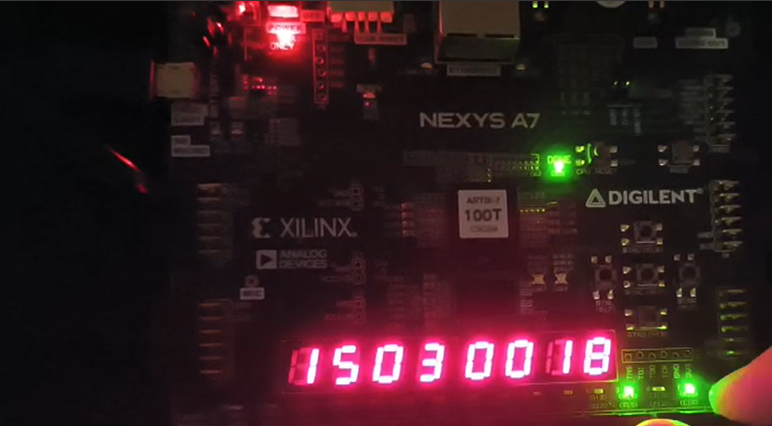
\includegraphics[width=0.6\textwidth]{suma.png}
  \caption{ADD con $A=15$ y $B=3$. Displays: A=\texttt{15} (AN7..AN6), B=\texttt{03} (AN5..AN4), Resultado=\texttt{0018} (AN3..AN0).}
  \label{fig:add}
\end{figure}


\subsection*{Resta (SUBTRACT)}
\begin{figure}[H]
  \centering
  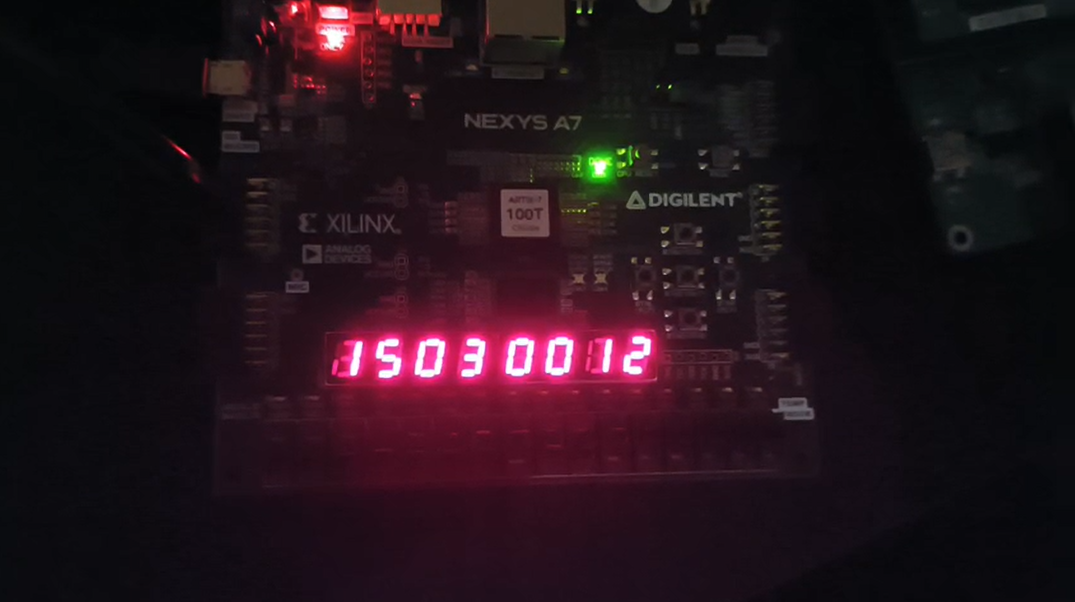
\includegraphics[width=0.6\textwidth]{resta.png}
  \caption{SUB con $A=15$ y $B=3$. Displays: A=\texttt{15}, B=\texttt{03}, Resultado=\texttt{0012} (hex bajo) pero mostrado como decimal \texttt{0012}}
  \label{fig:sub}
\end{figure}


\subsection*{Multiplicación (MULTIPLY)}
\begin{figure}[H]
  \centering
  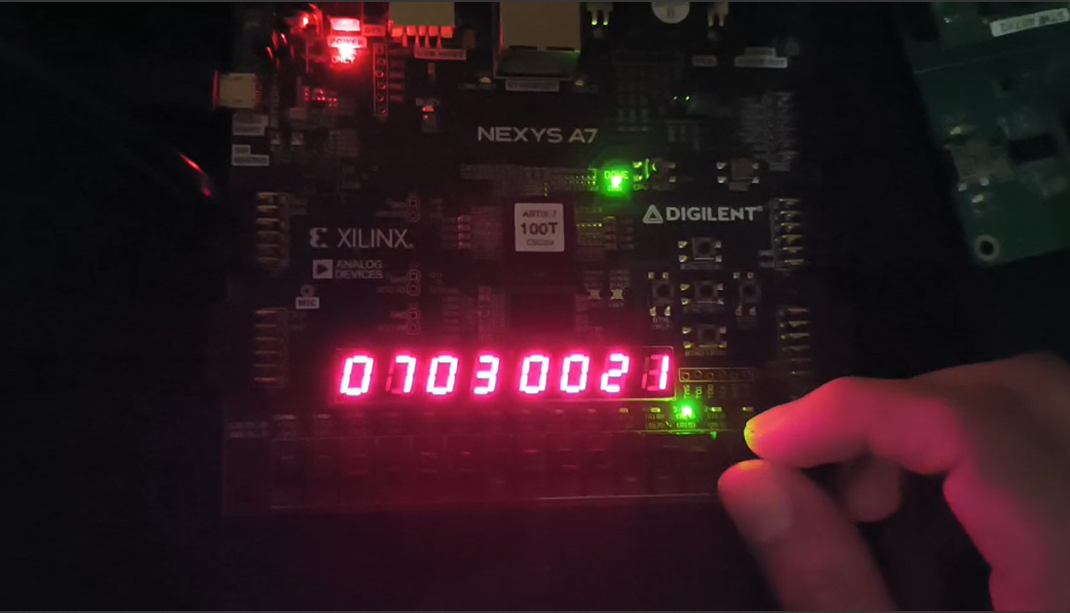
\includegraphics[width=0.6\textwidth]{mult.png}
  \caption{MUL con $A=7$ y $B=3$. Displays: A=\texttt{07}, B=\texttt{03}, Resultado=\texttt{0021}.}
  \label{fig:mul}
\end{figure}


\subsection*{División (DIVIDE)}
\begin{figure}[H]
  \centering
  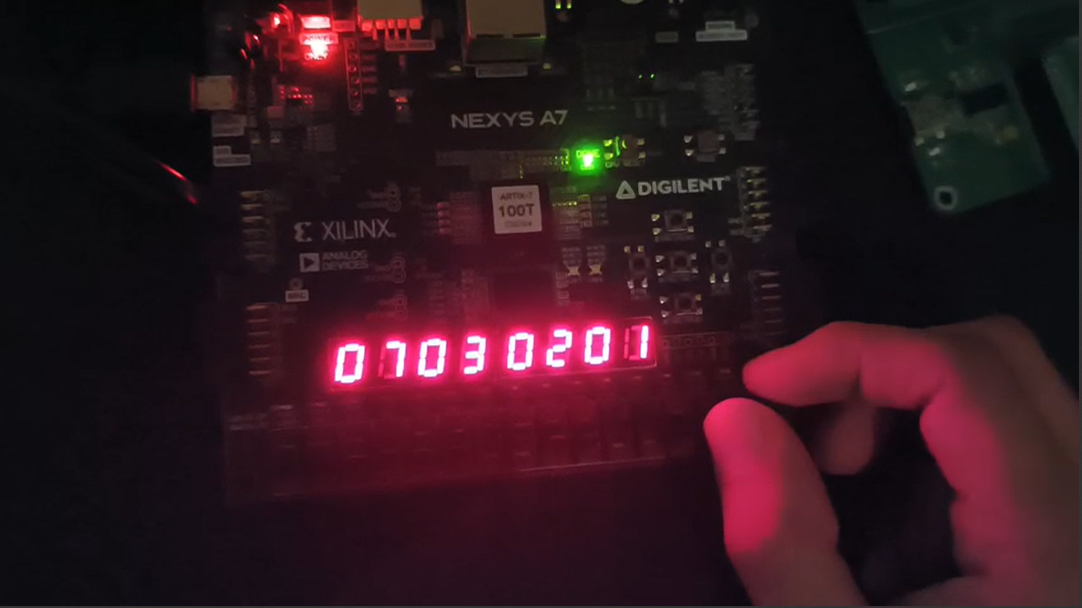
\includegraphics[width=0.6\textwidth]{div.png}
  \caption{DIV con $A=7$ y $B=3$. Displays: A=\texttt{07}, B=\texttt{03}, Resultado=\texttt{[Q=02][R=01]} en AN3..AN0.}
  \label{fig:div}
\end{figure}






\end{document}
